\chapter{The LMFL Laboratory}
%\chapter{CERFACS : Le fondement des logiciels de simulation numérique}
%\chapter*{Le CERFACS : Le fondement des logiciels de simulation numérique}
%\addcontentsline{toc}{chapter}{Le CERFACS : Le fondement des logiciels de
                                %simulation numérique}

% Faire les sous parties


%Le plan doit être dynamique : le lecteur doit ressentir une progression entre le début et la fin du rapport. Ainsi, la « présentation de l’entreprise » (partie I) doit permettre de mieux comprendre la « présentation du travail réalisé » (partie II). En effet, les choix industriels, les processus de fabrication, les méthodes de travail, l’organisation et la culture de l’entreprise, notamment en matière de responsabilité sociétale et de développement durable ( annexe IV, p. 39), ont nécessairement une incidence sur le travail
%du stagiaire.

% \section{Structure du CERFACS}

% \label{actionnaires}

The LMFL is a public laboratory under supervision of Centrale Lille, Université Lille 1, Arts et Métiers Paris Tech, ONERA and CNRS.

\begin{figure}[H]
    \centering
    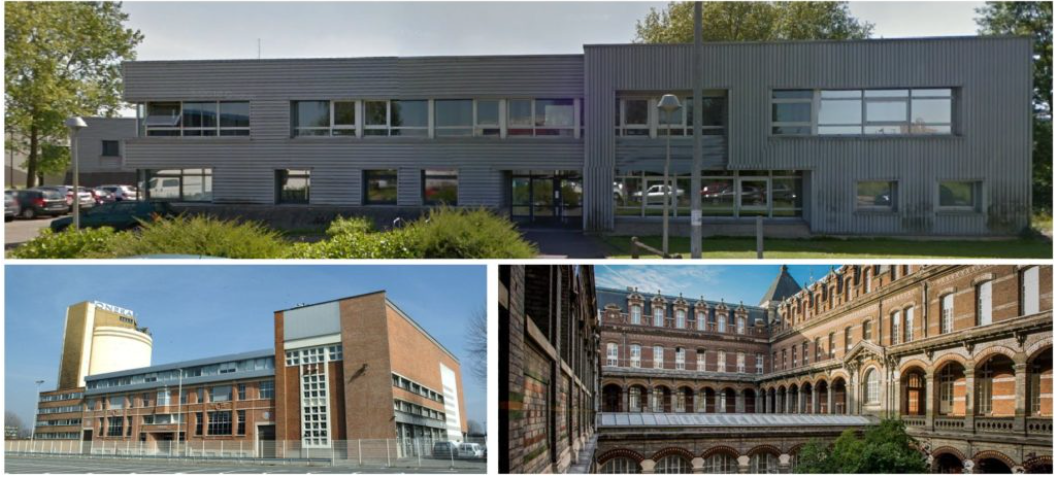
\includegraphics[width=0.90\textwidth]{images/LMFL_facilities.png}
    \caption{LMFL facilities; Top:Villeneuve d’Ascq’s campus gathering Centrale Lille,
    CNRS and Univsersité de Lille. Bottom-left: ONERA. Bottom-right: ENSAM (source : \href{https://lmfl.cnrs.fr/le-laboratoire/}{lmfl.cnrs.fr})}
    %\label{fig:autocorrelation}
\end{figure}



During the last six months, I have been hosted by École Nationale Supérieure des Arts et
Métiers (ENSAM), more precisely at Lille campus. Arts et Métiers is known to be a
prestigious engineering school with a focus on mechanics, industrial and energy engineering.
Its Lille campus offers students unique opportunities to study in a dynamic and innovative
environment, located in the heart of a region known for its industrial history.

This research structure was created on January 1, 2018 by the merger of two research units: the “Écoulements tournants et turbulents” team at the Lille Mechanics Laboratory, and the “Expérimentation et Limite de Vol” research unit.


% (Algorithmes Parallèles \& sCientifics sOftware Operational Performances)
% (Équipe Informatique et Support Utilisateur)
% (Energy et Safety)
% (Advanced Aerodynamics and Multiphysics)
% (Modélisation du climat et de son changement global)

% \section{Mon équipe}

This diversity of skills allows the research teams to be involved in numerous partnership
projects in connection with regional or national structures.
Research conducted within the LMFL is organized into three main topics:
\begin{itemize}
    \item \textbf{Turbulence} : Studying and modeling turbulent flows using numerical and experimental methods. A focus is made on inhomogeneity and non-stationarity in
    wall-bounded flows, wakes, jets and several other flow configurations. This research
    theme gathers 5 permanent researchers and about 10 PhD and post-doctoral
    students.
    \item \textbf{Rotating flows} (CFD) : Analyzing and modeling internal and external flows related to rotating machines, such as turbo-machinery and rotors. Experimental and numerical study of rotating machines (turbomachines, rotors, propellers) operating in degraded conditions, flow control, cavitation and multiphase flows are also topics of great interest.
    This subject gathers 6 researchers, 7 research engineers and about 13 PhD and post-
    doctoral students.
    \item \textbf{Flight dynamics in unsteady and non-uniform environments} : Development of analytical and experimental methods to determine the evolving behaviour of low-speed aircrafts in perturbed flight domains. Dynamic of post-stall behaviour, interaction with the environment and definition of experiments are subjects of interest. This topic gathers about 5 research engineers and 5 PhD and post-doctoral students.
\end{itemize}


La \ac{CAO} permet de faire les plans numériques d'un avion par exemple, afin de s'assurer que toutes les pièces fabriquées vont bien s'imbriquer entre elles. Mais cela permet aussi de faire des simulations numériques pour prévoir la tenue structurelle, les forces aérodynamiques, le volume sonore, etc. sans avoir à faire d'onéreux tests.

L'équipe AAM se focalise sur la simulation des écoulements aérodynamiques externes en développant des méthodes numériques avancées et en les appliquant aux avions, fusées, hélicoptères, moteurs, turbomachines, etc.
Les liens de l’équipe AAM avec toutes les autres équipes du CERFACS sont forts.
Par exemple, les simulations des chambres de combustion faites par l'équipe ES donnent les conditions de sortie dans des moteurs d'avions qui sont ensuite utilisées par l'équipe AAM pour des simulations aéroacoustique.
Dans l'autre sens, les simulations aérodynamiques externes des ailes d'avions réalisés par AAM sont ensuite utilisées à GLOBC pour faire des analyses des contrails afin de déterminer leur impact sur le climat.


Le CERFACS héberge des supercalculateurs et un serveur sur lequel se trouve l'intranet avec toutes les ressources nécessaires aux employés.  % (Kraken, Calypso et Scylla)   % Scylla, est un calculateur utilisé par globc pour les post traitement de grandes volumes de données météo
Nous y trouvons notamment les liens vers la \ac{QVT}, le \ac{CSE}, un document "Plan du management de la qualité" ainsi que de nombreuses autres ressources.
%Le \ac{CSSCT} et le \ac{DUERP} devraient obligatoirement y être présents selon le site du gouvernement. % détailler


%\newpage

% \section{La RSE au CERFACS}

Après une recherche non fructueuse sur l'intranet, j'ai pu demander à la responsable des ressources humaines le document relatant des objectifs \ac{RSE}. Le document d'actions RSE est segmenté en trois parties principales :

\paragraph{Démarche RSE}

%En voici le contenu :

https://artsetmetiers.fr/fr/ecole-engagee
https://artsetmetiers.fr/fr/actualites/developpement-durable-et-rse-faites-le-plein-de-connaissances-sur-savoir
https://savoir.ensam.eu/moodle/course/view.php?id=2793


\begin{quote}
\setlength{\leftmargin}{0.5cm} % Ajuster la marge gauche
\setlength{\rightmargin}{0.5cm} % Ajuster la marge droite
    "Le Cerfacs n’a pas mis en place une démarche spécifique RSE mais des actions ont été réalisées dans
    ce cadre, vis-à-vis de l’écoresponsabilité, la qualité de vie au travail et une charte éthique a été
    incluse dans le règlement intérieur depuis décembre 2023 (intégrant notamment la prévention de la
    corruption et la gestion des conflits d’intérêts).

    En outre, le Cerfacs achète ses fournitures auprès de créateurs solidaires (exemple : Antilope qui
    compte 32 salariés sur les 49 avec une reconnaissance de « travailleur handicapé »).

    Le Cerfacs met à jour au moins deux fois par an et aussi souvent que nécessaire un document unique
    d’évaluation des risques Cerfacs (avec un plan d’actions de prévention).

    Le Cerfacs a nommé des référents : un référent « Santé et Sécurité », un référent « \ac{RGPD} », un
    référent « Handicap », deux référents « Harcèlement, agissements sexistes et violences ».

    Un bilan HSE et RSE est présenté chaque année aux Associés du Cerfacs lors de l’Assemblée d’avril."
\end{quote}



\paragraph{Écoresponsabilité}
\hspace{0,5cm}

    J'ai constaté beaucoup d'actions dans le sens de l'écoresponsabilité lors de mon stage. La plupart sont mentionnées dans le document d'actions RSE.

    %Un Groupe de Travail « Bilan carbone du CERFACS », composé de 10 volontaires, a été créé. Des bilans carbone ont été réalisés pour les années 2019 et 2021, en suivant la méthodologie proposée par le collectif de laboratoires Labos1point5\footnote{\url{https://labos1point5.org}}. Depuis mi-2023, le CERFACS collabore avec le Cabinet Take[air]\footnote{\url{https://www.takeair.fr/}} pour établir un plan d’actions visant à réduire son empreinte carbone. Cette collaboration a permis de réaliser le bilan carbone de 2022 et de commencer l'élaboration d'un plan d'action, qui devrait être finalisé à l’automne 2024, après la tenue de plusieurs ateliers. Finalement nous trouvons dans le document un tableau \annexref{tab:Eco_actions} récapitulant les principaux postes d'émission identifiés dans une première colonne puis les objectifs et actions associées dans une seconde colonne.

    En parallèle, j'ai entendu parler de cette démarche en discutant avec des thésards. Et j'ai aussi pu trouver la page depuis l'intranet. Elle est divisée en cinq sections : "présentation", "actualités", "émissions", "bilan" et "actions".
    %J'aime beaucoup l'image ci-dessous (figure \ref{fig:evolution_empreinte_carbone}), présente dans le document et le site internet, qui montre que le CERFACS réduit ses émissions d'année en année. Cela est probablement lié aux efforts du groupe « Bilan carbone du CERFACS ». L'année 2021 est peu représentative, car grandement marquée par une diminution des missions à cause de la COVID. Mais 2022 nous montre bien que le CERFACS réduit les émissions dues à ses missions, à la fabrication et utilisation de calculateurs externes, aux trajets domicile-travail et au matériel informatique, sujets cibles de la sensibilisation menée par le groupe.

    %\begin{figure}[H]
    %    \centering
    %    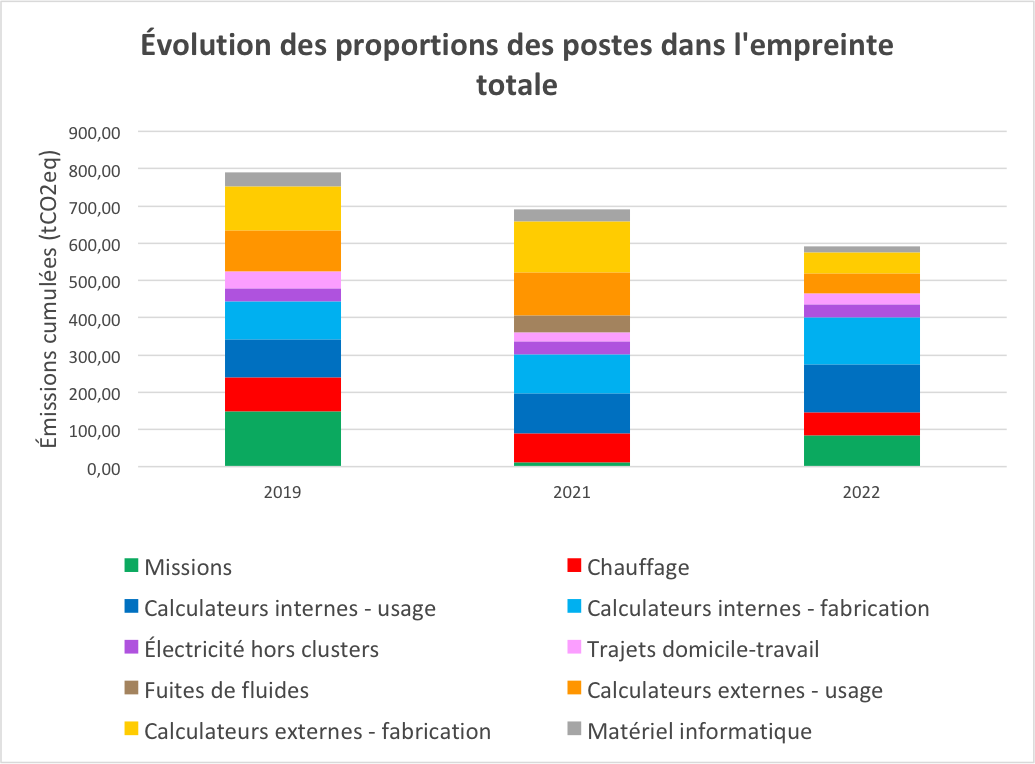
\includegraphics[width=0.85\textwidth]{images/evolution_postes_empreintecarbone.png}
    %    \caption{Évolution de l'empreinte carbone du CERFACS entre 2019 et 2022}
    %    \label{fig:evolution_empreinte_carbone}
    %\end{figure}

    Dans les couloirs du CERFACS, on trouve des posters très clairs sur l'empreinte carbone d'un trajet pour une conférence en fonction des moyens de transport.
    Les employés sont incités à venir à vélo. Le CERFACS donne une prime pour chaque kilomètre fait à vélo sur le trajet domicile-travail. Il y a aussi un atelier de réparation et des emplacements sécurisés pour les vélos.
    La politique de communication n'est pas spécialement tournée vers les efforts pour le climat ou la RSE, mais le CERFACS agit efficacement en ce sens.

\paragraph{Responsabilité sociale / Qualité de vie au travail}
    \begin{quote}
        \setlength{\leftmargin}{0.5cm} % Ajuster la marge gauche
        \setlength{\rightmargin}{0.5cm} % Ajuster la marge droite
        "La démarche Qualité de Vie au Travail (QVT) a été lancée au Cerfacs en janvier 2022, avec la mise en
        place d’un Groupe de Travail : elle a permis d’identifier 6 axes de travail pour améliorer le
        fonctionnement de la structure et du ressenti des personnes :
        \begin{itemize}
            \item Optimiser l’organisation et gestion du travail au niveau global
            \item Optimiser l’organisation et gestion du travail au niveau de l’équipe
            \item Optimiser l’organisation et gestion du travail au niveau personnel
            \item Assurer un meilleur accueil et support des non permanents
            \item Favoriser la vie sociale
            \item Améliorer le confort matériel"
        \end{itemize}
    \end{quote}

    %De nouveau, un tableau \annexref{tab:QVT_actions} détaille des exemples d'actions que j'ai pu expérimenter (salle de repos, machine à café, parking vélo, etc.).

    Un dernier plan d'action a été mis en place sur l'égalité professionnelle entre les femmes et les hommes. Il traite de divers sujets : l’embauche, la rémunération effective, l’articulation entre l’activité professionnelle et l’exercice de la responsabilité familiale.

    Je tiens à mentionner également que j'ai reçu un mail qui lançait un appel au volontariat pour composer le Comité de Pilotage pour la Prévention des Violences Sexistes et Sexuelles au Travail suite à une réunion d'information réalisée en collaboration avec la médecine du travail.

\newpage


Mon ressenti personnel sur le cadre de travail est très positif. Être assis dans un bureau climatisé avec une vue sur la campagne participe évidemment à cela. Un des seuls risques à ce type de travail est une mauvaise position qui peut entraîner des troubles musculosquelettiques. Pour pallier cela, il y a des affiches dans chaque bureau indiquant la meilleure position à avoir et proposant des exercices. Ces mêmes informations apparaissent dans le 'livret d'accueil stagiaire' qui m'a été remis le premier jour.
Une cantine présente sur le site à quelques minutes à pied, permet de déjeuner et échanger avec les collègues du CERFACS hors cadre professionnel.